% Informe tecnico en formato APA 7. Compilar con XeLaTeX y biber.
\documentclass[stu,letterpaper,floatsintext,nolmodern,nofontenc]{apa7}

\usepackage{fontspec}
\setmainfont{Times New Roman}
\setmonofont{Consolas}
\usepackage[spanish,es-noshorthands]{babel}
\usepackage{csquotes}
\usepackage{indentfirst}
\usepackage{etoolbox}
\usepackage{array}
\usepackage{longtable}
\usepackage{float}
\usepackage{booktabs}
\usepackage{listings}

\usetikzlibrary{positioning,arrows.meta,shapes.geometric}

\usepackage[style=apa,backend=biber]{biblatex}
\addbibresource{informe-medicontrol.bib}
\hypersetup{hidelinks}

\hyphenpenalty=10000
\exhyphenpenalty=10000

\lstdefinelanguage{Dart}{
  morekeywords={async,await,break,case,catch,class,const,continue,default,do,else,enum,extends,false,final,finally,for,if,import,in,is,new,null,return,super,switch,this,throw,true,try,var,void,while},
  sensitive=true,
  morecomment=[l]{//},
  morestring=[b]',
  morestring=[b]"
}
\lstset{
  language=Dart,
  basicstyle=\ttfamily\linespread{1}\fontsize{8}{9.6}\selectfont,
  breaklines=true,
  columns=fullflexible,
  keepspaces=true,
  showstringspaces=false,
  frame=leftline,
  framerule=0.4pt,
  xleftmargin=1em,
  aboveskip=1pt,
  belowskip=1pt,
  keywordstyle=\bfseries,
  stringstyle={}
}
\begingroup
\catcode`\%=12
\lstset{literate={%}{\char37}1}
\endgroup

\tikzset{
  mcbox/.style={draw=black, rounded corners=1pt, fill=gray!12, align=center,
    inner sep=2.2pt, font=\scriptsize},
  mcdia/.style={diamond, draw=black, fill=gray!12, aspect=2.5, align=center,
    inner sep=0.6pt, font=\scriptsize},
  mcarr/.style={-{Stealth[length=1.4mm]}, draw=black, thin}
}

\makeatletter
\patchcmd{\maketitle}{\vspace*{4\baselineskip}}{%
  
\includegraphics[width=2.45cm]{figuras/logo-unifranz.png}\\[0.6\baselineskip]
}{}{%
  \PackageWarning{medicontrol}{No se pudo insertar el logo en la portada}%
}
\makeatother

\setlength{\intextsep}{6pt plus 2pt minus 2pt}
\setlength{\textfloatsep}{6pt plus 2pt minus 2pt}
\setlength{\floatsep}{6pt plus 2pt minus 2pt}

\title{Informe técnico de la aplicación MediControl}
\shorttitle{Informe técnico de MediControl}
\authorsnames{Miguel Angel Andrade Arnez}
\authorsaffiliations{Universidad Franz Tamayo, Facultad de Ingeniería, Carrera de Ingeniería de Sistemas}
\course{Sistemas Operativos Móviles y Embebidos}
\professor{Ing. Christian Luis Lopez Bravo}
\duedate{6 de octubre de 2026}

\begin{document}
\maketitle

\section{Introducción, Objetivo y Entorno}

MediControl digitaliza la gestión de pacientes y citas de una clínica.
Esta entrega corresponde al Hito 3, tarea A3.2, avance del proyecto procesual.
El objetivo es que el personal consulte y registre esa información en el dispositivo, sin depender de cuadernos.

El entorno es Flutter 3.44.7, Dart 3.12.2, Android SDK 36 y JDK 17 de Microsoft \parencite{flutterDocs}.
El emulador es \path{MediControl_liviano}, un Pixel 3a con 2 GB de RAM.
No se usa Android Studio. Desde \path{medicontrol/} se ejecuta:

{\linespread{1}\selectfont
\begin{lstlisting}[language={}]
flutter pub get
flutter emulators --launch MediControl_liviano
flutter run
\end{lstlisting}}

\section{Alcance por Módulo}

Lo implementado en esta entrega cubre seis módulos. El resto queda como trabajo futuro.
La sincronización con Firebase o una API todavía no está.

\begin{table}[H]
\caption{Módulos implementados en esta entrega y trabajo futuro}
\centering
{\linespread{1}\selectfont\footnotesize
\begin{tabular}{@{}>{\raggedright\arraybackslash}p{2.15cm}>{\raggedright\arraybackslash}p{6.7cm}>{\raggedright\arraybackslash}p{6.5cm}@{}}
\toprule
Módulo & Implementado en esta entrega & Trabajo futuro \\
\midrule
Login & Correo y contraseña de demostración; la sesión queda en el dispositivo & Recuperar contraseña \\
Inicio & Accesos rápidos y la próxima cita & Recordatorios \\
Pacientes & Listar, buscar y dar de alta & --- \\
Perfil & Datos, consultas pasadas y un tratamiento de ejemplo (texto fijo) & Historial clínico editable y CRUD de tratamientos \\
Agenda & Calendario del mes y citas del día elegido & --- \\
Nueva cita & Paciente, fecha, hora y motivo; la cita debe ser futura & --- \\
\bottomrule
\end{tabular}}
\end{table}

El usuario de demostración es \path{miguel@clinicademo.com} con la contraseña \path{demo1234}.

\section{Arquitectura}

Las pantallas no hablan con SQLite.
La carpeta \path{features/} usa \path{AuthController} y \path{ClinicaController}, ambos \path{ChangeNotifier} \parencite{changeNotifier,providerPkg}.
Esos controladores dependen de \path{AuthRepository}, \path{PacienteRepository} y \path{CitaRepository}.
Hoy las implementaciones son locales: \path{LocalAuthRepository} guarda la sesión con \path{shared_preferences} y \path{LocalPacienteRepository} junto con \path{LocalCitaRepository} usan sqflite \parencite{sharedPrefs,sqflitePkg}.
La línea punteada de la Figura 1 reserva el mismo contrato para un backend remoto.
\path{lib/} reúne 35 archivos Dart y cerca de 2\,400 líneas.
La sección Estructura de carpetas dice qué hay en cada ruta.

\begin{figure}[H]
\caption{Capas de MediControl. La línea punteada es trabajo futuro}
\centering
{\linespread{1}\selectfont
\begin{tikzpicture}
  \node[mcbox, text width=11.6cm] (fe) at (0,0) {features (pantallas)};
  \node[mcbox, text width=11.6cm] (co) at (0,-0.78) {AuthController y ClinicaController (ChangeNotifier)};
  \node[mcbox, text width=11.6cm] (re) at (0,-1.56) {AuthRepository, PacienteRepository y CitaRepository};
  \node[mcbox, text width=11.6cm] (lo) at (0,-2.34) {LocalAuthRepository (shared\_preferences) y Local*Repository (sqflite)};
  \node[mcbox, dashed, text width=11.6cm] (fu) at (0,-3.12) {futuro: Firebase o API};
  \draw[mcarr] (fe) -- (co);
  \draw[mcarr] (co) -- (re);
  \draw[mcarr] (re) -- (lo);
  \draw[mcarr, dashed] (lo) -- (fu);
\end{tikzpicture}}
\end{figure}

\section{Estructura de Carpetas}

La Tabla~\ref{tab:carpetas} recorre las rutas reales.
Salvo \path{figuras/} y el informe APA anterior, las rutas son relativas a \path{medicontrol/}.
\path{aplicacion-medicontrol.tex} y su PDF describen la aplicación prevista; no son el código.
Las cuatro últimas filas las generan Flutter, la compilación, el IDE o Gradle: no forman parte del código que se mantiene a mano.

\begingroup
\linespread{1}\fontsize{8}{9.6}\selectfont
\setlength{\tabcolsep}{3pt}
\begin{longtable}{@{}>{\raggedright\arraybackslash}p{4.05cm}>{\raggedright\arraybackslash}p{5.45cm}>{\raggedright\arraybackslash}p{6.05cm}@{}}
\caption{Carpetas del repositorio y del paquete MediControl}\label{tab:carpetas}\\
\toprule
Carpeta & Contenido & Para qué sirve \\
\midrule
\endfirsthead
\toprule
Carpeta & Contenido & Para qué sirve \\
\midrule
\endhead
\midrule
\endfoot
\bottomrule
\endlastfoot
\path{figuras/} & \path{logo-unifranz.png}, \path{interfaz-medicontrol.png} & Escudo e interfaz del informe anterior \\
\path{aplicacion-medicontrol.tex} y \path{.pdf} & Informe APA previo & Describe la idea; no es la aplicación \\
\path{android/} & \path{app/} (manifiesto, \path{MainActivity.kt}, \path{res/}), \path{gradle.properties}, wrapper & Proyecto Gradle que empaqueta la app \\
\path{lib/} & \path{main.dart}, \path{app.dart}, \path{core/}, \path{data/}, \path{features/}, \path{widgets/} & Código Dart que se mantiene a mano \\
\path{lib/core/} & \path{consultas.dart}, \path{validators.dart} & Reglas de citas y validación, sin pantallas \\
\path{lib/core/format/} & \path{fechas.dart} & Comparar días y formatear fechas \\
\path{lib/core/router/} & \path{app_router.dart} & Rutas, shell y redirect de sesión \\
\path{lib/core/theme/} & \path{app_theme.dart} & Colores y tema visual \\
\path{lib/data/} & \path{models/}, \path{local/}, \path{repositories/} & Entidades, base local y contratos \\
\path{lib/data/models/} & \path{paciente.dart}, \path{cita.dart}, \path{usuario.dart} & Entidades en memoria \\
\path{lib/data/local/} & \path{app_database.dart}, \path{semilla.dart}, \path{session_store.dart} & SQLite, datos de demo y claves de sesión \\
\path{lib/data/repositories/} & Contrato y clase local de auth, paciente y cita (6 archivos) & Acceso local y enchufe para un backend \\
\path{lib/features/} & auth, home, clinica, pacientes, perfil, agenda, citas, mas, proximamente & Una carpeta por módulo de la interfaz \\
\path{lib/features/auth/} & \path{login_screen.dart}, \path{auth_controller.dart} & Formulario de acceso y estado de sesión \\
\path{lib/features/home/} & \path{home_screen.dart} & Inicio, accesos y próxima cita \\
\path{lib/features/clinica/} & \path{clinica_controller.dart} & Catálogo, lista filtrada y agenda \\
\path{lib/features/pacientes/} & \path{pacientes_screen.dart}, \path{paciente_form_screen.dart} & Listado, búsqueda y alta \\
\path{lib/features/perfil/} & \path{perfil_screen.dart}, \path{tratamiento_fijo.dart} & Ficha, citas pasadas y texto fijo \\
\path{lib/features/agenda/} & \path{agenda_screen.dart} & Calendario mensual y citas del día \\
\path{lib/features/citas/} & \path{cita_form_screen.dart} & Alta de una cita futura \\
\path{lib/features/mas/} & \path{mas_screen.dart} & Usuario activo y cierre de sesión \\
\path{lib/features/proximamente/} & \path{proximamente_screen.dart} & Aviso de historial y de tratamientos \\
\path{lib/widgets/} & \path{app_shell.dart}, \path{cita_tile.dart}, \path{paciente_tile.dart}, \path{tarjeta.dart} & Barra inferior y piezas reutilizables \\
\path{test/} & \path{validadores_test.dart}, \path{modelos_test.dart}, \path{clinica_test.dart}, \path{widget_test.dart} & Pruebas automáticas del paquete \\
\path{test/soporte/} & \path{fakes.dart} & Sesión y repositorios en memoria \\
\path{capturas/} & \path{01-login.png} a \path{05-agenda.png} & Cinco pantallas del emulador \\
\path{lib/main.dart} & función \path{main} & Abre la base, carga la sesión y arranca \\
\path{lib/app.dart} & \path{MediControlApp} & Provider, idioma español y router \\
\path{pubspec.yaml} & Dependencias y SDK \path{^3.12.2} & Manifiesto del paquete \\
\path{pubspec.lock} & Versiones resueltas & Fija lo que se compiló \\
\path{analysis_options.yaml} & \path{include} de flutter\_lints & Reglas de \path{flutter analyze} \\
\path{README.md} & Requisitos, usuario demo y comandos & Cómo correr el paquete \\
\path{.gitignore} & Ignora \path{.dart_tool/}, \path{build/} y \path{.idea/} & Excluye generados del paquete \\
\path{.dart_tool/} & \path{package_config.json}, \path{package_graph.json}, \path{flutter_build/} & La genera Flutter; no se mantiene a mano \\
\path{build/} & \path{app/}, \path{.cxx/}, \path{reports/} & La genera la compilación; no se mantiene a mano \\
\path{.idea/} & \path{modules.xml}, \path{workspace.xml}, \path{runConfigurations/} & La genera el IDE; no se mantiene a mano \\
\path{android/.gradle/} & Caché \path{9.1.0/} y \path{buildOutputCleanup/} & La genera Gradle; no se mantiene a mano \\
\end{longtable}
\endgroup

\section{Navegación y Modelo de Datos}

\path{go_router} abre en \path{/inicio} y el redirect manda a \path{/login} si no hay sesión \parencite{goRouter}.
La barra inferior es un \path{StatefulShellRoute} con cuatro ramas: \path{/inicio}, \path{/pacientes}, \path{/citas} y \path{/mas}.
Fuera del shell quedan \path{/paciente/nuevo}, \path{/paciente/:id}, \path{/cita/nueva}, \path{/historial} y \path{/tratamientos}.
Historial y tratamientos muestran \path{ProximamenteScreen}.

\begin{figure}[H]
\caption{Rutas: login, cuatro ramas del shell y pantallas fuera del shell}
\centering
{\linespread{1}\selectfont
\begin{tikzpicture}
  \node[mcbox] (login) at (0,0) {/login};
  \node[mcbox, text width=12.2cm] (shell) at (0,-1.05)
    {shell: /inicio \quad /pacientes \quad /citas \quad /mas};
  \node[mcbox, text width=12.2cm, align=center] (out) at (0,-2.25)
    {fuera: /paciente/nuevo \quad /paciente/:id \quad /cita/nueva\\
     /historial \quad /tratamientos};
  \draw[mcarr] (login) -- (shell);
  \draw[mcarr] (shell) -- (out);
\end{tikzpicture}}
\end{figure}

Cada paciente tiene varias citas. La clave foránea es \path{paciente_id}.
La sesión no está en SQLite: \path{PreferenciasSesion} escribe \path{sesion_id}, \path{sesion_nombre} y \path{sesion_correo}.
Si \path{pacientes} está vacía, \path{AppDatabase.abrir} llama a \path{crearSemilla(DateTime.now())}.
Entran Juan Pérez, María López, Carlos Andrade, Ana Torres y Luis Fernández, con citas de hoy, de mañana, dentro de tres días y varias pasadas (entre ellas $-6$ y $-14$ días).

\begin{figure}[H]
\caption{Pacientes, citas y las tres claves de sesión}
\centering
{\linespread{1}\selectfont
\begin{tikzpicture}
  \node[mcbox, align=left, font=\scriptsize, text width=6.3cm] (pac) at (0,0)
    {\textbf{pacientes}\\
     id INTEGER PK\\
     nombre, ci UNIQUE, telefono\\
     fecha\_nacimiento, direccion, activo};
  \node[mcbox, align=left, font=\scriptsize, text width=5.6cm] (cit) at (7.4,0)
    {\textbf{citas}\\
     id INTEGER PK\\
     paciente\_id INTEGER FK\\
     fecha\_hora, motivo, notas};
  \node[mcbox, align=left, font=\scriptsize] (ses) at (3.6,-2.15)
    {\textbf{shared\_preferences}\\
     sesion\_id, sesion\_nombre, sesion\_correo};
  \draw[mcarr] (pac) -- node[above, font=\scriptsize] {1--N} (cit);
\end{tikzpicture}}
\end{figure}

\section{Lógica de Programación}

\subsection{Arranque y Sesión}

\path{main} inicializa el idioma \path{es_ES}, abre la base (y siembra si está vacía), crea el controlador de autenticación y llama a \path{cargarSesion}.
Esa lectura de tres claves es el mismo uso de SharedPreferences del Hito 3: si existen, el redirect deja pasar a \path{/inicio}; si no, devuelve \path{/login}.
\path{refreshListenable} vuelve a evaluar el redirect cuando la sesión cambia.

\begin{figure}[H]
\caption{Arranque: si la base está vacía se siembra y, si hay sesión, se abre el inicio}
\centering
{\linespread{1}\selectfont
\begin{tikzpicture}
  \node[mcbox] (a) at (0,0) {abre la base};
  \node[mcdia] (v) at (2.55,0) {¿vacía?};
  \node[mcbox] (s) at (5.05,0) {siembra};
  \node[mcbox] (c) at (7.7,0) {cargarSesion};
  \node[mcdia] (h) at (10.35,0) {¿sesión?};
  \node[mcbox] (i) at (12.7,0) {/inicio};
  \node[mcbox] (l) at (12.7,-1.15) {/login};
  \draw[mcarr] (a) -- (v);
  \draw[mcarr] (v) -- node[above, font=\scriptsize] {sí} (s);
  \draw[mcarr] (s) -- (c);
  \draw[mcarr] (v.south) to[out=-80, in=-100] node[below, font=\scriptsize] {no} (c.south);
  \draw[mcarr] (c) -- (h);
  \draw[mcarr] (h) -- node[above, font=\scriptsize] {sí} (i);
  \draw[mcarr] (h.south) -- node[right, font=\scriptsize] {no} (l.north);
\end{tikzpicture}}
\end{figure}

{\linespread{1}\selectfont
\begin{lstlisting}
        return enLogin ? null : '/login';
      }
      if (enLogin) {
        return '/inicio';
\end{lstlisting}}

\subsection{Autenticación Local}

\path{LocalAuthRepository} recorta el correo, lo pasa a minúsculas y lo compara con \path{CredencialesDemo}.
Si no coincide, lanza \path{CredencialesInvalidas} y la pantalla de login muestra el error.
La contraseña va en texto plano a propósito, solo en memoria: la sesión guardada no la incluye.

\subsection{Reglas de Citas}

\path{proximaCita}, \path{citasEnDia} e \path{historialPaciente}, en \path{consultas.dart}, son funciones puras: no abren la base, y por eso se prueban con listas.
\path{proximaCita} devuelve la cita con \path{fechaHora} más temprana que no sea anterior a ahora.
\path{citasEnDia} filtra con \path{mismoDia} y ordena por hora.
\path{historialPaciente} deja las citas pasadas de ese paciente, de la más reciente a la más antigua.

{\linespread{1}\selectfont
\begin{lstlisting}
    if (cita.fechaHora.isBefore(ahora)) {
      continue;
    }
    if (proxima == null || cita.fechaHora.isBefore(proxima.fechaHora)) {
\end{lstlisting}}

\subsection{Búsqueda de Pacientes}

El listado usa \path{LIKE} con \path{ESCAPE} sobre el nombre o el CI.
\path{_like} escapa la barra, el porcentaje y el guion bajo para que el texto escrito no actúe como comodín.
\path{ClinicaController} guarda el catálogo completo en \path{catalogo} y la lista filtrada en \path{lista}: el formulario de citas sigue viendo a todos.

{\linespread{1}\selectfont
\begin{lstlisting}
            where: "nombre LIKE ? ESCAPE '\\' OR ci LIKE ? ESCAPE '\\'",
            whereArgs: [_like(texto), _like(texto)],
\end{lstlisting}}

{\linespread{1}\selectfont
\begin{lstlisting}
      .replaceAll(r'\', r'\\')
      .replaceAll('%', r'\%')
      .replaceAll('_', r'\_');
  return '%$limpio%';
\end{lstlisting}}

\subsection{Validación}

\begin{table}[H]
\caption{Reglas de los formularios}
\centering
{\linespread{1}\selectfont\footnotesize
\begin{tabular}{@{}>{\raggedright\arraybackslash}p{2.3cm}>{\raggedright\arraybackslash}p{4.4cm}>{\raggedright\arraybackslash}p{8.6cm}@{}}
\toprule
Campo & Regla & Mensaje \\
\midrule
Correo & Vacío o sin formato & Ingresa el correo electrónico / El correo no tiene un formato válido \\
Contraseña & Al menos 6 caracteres & La contraseña debe tener al menos 6 caracteres \\
CI & 5 a 10 dígitos y único & El CI debe tener entre 5 y 10 dígitos. Si ya existe: Ya existe un paciente con ese CI (\path{CiDuplicado}) \\
Teléfono & 7 a 12 dígitos & El teléfono debe tener entre 7 y 12 dígitos \\
\bottomrule
\end{tabular}}
\end{table}

\subsection{Guardar una Cita}

El formulario tiene que ser válido, con fecha y hora elegidas.
Esas partes se arman en un \path{DateTime}.
Si no queda en el futuro, no se guarda.
Si pasa, \path{agregarCita} inserta y \path{refrescar} vuelve a leer la base.
Agenda e Inicio observan al controlador y se actualizan solos.

\begin{figure}[H]
\caption{Comprobaciones al guardar una cita y camino de error}
\centering
{\linespread{1}\selectfont
\begin{tikzpicture}
  \node[mcbox] (form) at (0,0) {formulario};
  \node[mcdia] (val) at (0,-1.45) {¿válido?};
  \node[mcbox] (e1) at (3.5,-1.45) {error};
  \node[mcdia] (hora) at (0,-2.9) {¿hora?};
  \node[mcbox] (e2) at (3.5,-2.9) {error};
  \node[mcdia] (fut) at (0,-4.35) {¿futuro?};
  \node[mcbox] (e3) at (3.5,-4.35) {error};
  \node[mcbox] (ok) at (0,-5.7) {agregarCita y refrescar};
  \draw[mcarr] (form) -- (val);
  \draw[mcarr] (val) -- node[above, font=\scriptsize] {no} (e1);
  \draw[mcarr] (val) -- node[right, font=\scriptsize] {sí} (hora);
  \draw[mcarr] (hora) -- node[above, font=\scriptsize] {no} (e2);
  \draw[mcarr] (hora) -- node[right, font=\scriptsize] {sí} (fut);
  \draw[mcarr] (fut) -- node[above, font=\scriptsize] {no} (e3);
  \draw[mcarr] (fut) -- node[right, font=\scriptsize] {sí} (ok);
\end{tikzpicture}}
\end{figure}

{\linespread{1}\selectfont
\begin{lstlisting}
    if (!fechaHora.isAfter(DateTime.now())) {
      setState(() => _error = 'La cita debe quedar en el futuro');
      return;
    }
\end{lstlisting}}

\subsection{Ciclo con Provider}

La pantalla llama al controlador con \path{context.read}.
El controlador usa el repositorio, la base cambia y \path{notifyListeners} avisa.
Quien hizo \path{context.watch} se redibuja.
Por eso una cita nueva aparece en la agenda y en el inicio sin código extra entre esas pantallas.

\begin{figure}[H]
\caption{Ciclo de estado: la pantalla pide, la base cambia y watch redibuja}
\centering
{\linespread{1}\selectfont
\begin{tikzpicture}
  \node[mcbox] (p) at (0,0) {Pantalla};
  \node[mcbox] (c) at (3.5,0) {Controlador};
  \node[mcbox] (r) at (7.3,0) {Repositorio};
  \node[mcbox] (b) at (10.8,0) {sqflite};
  \draw[mcarr] (p) -- node[above, font=\scriptsize] {read} (c);
  \draw[mcarr] (c) -- (r);
  \draw[mcarr] (r) -- (b);
  \draw[mcarr] (c.south) .. controls +(0,-0.85) and +(0,-0.85) ..
    node[below, font=\scriptsize] {notifyListeners y watch} (p.south);
\end{tikzpicture}}
\end{figure}

\subsection{Semilla Relativa}

\path{crearSemilla(ahora)} calcula cada cita con \path{dia(offset, hora, minuto)} respecto del día de instalación.
Así la agenda y la próxima cita tienen contenido el día en que se instala la aplicación.

\section{Librerías y Configuración}

Las versiones son las resueltas en \path{pubspec.lock} a partir de \path{pubspec.yaml}.
\path{intl} quedó fijo en 0.20.2 porque lo exige \path{flutter_localizations}; por eso \path{table_calendar} es 3.2.1 y no 3.3.0 \parencite{intlPkg,tableCalendar}.

\begin{table}[H]
\caption{Librerías directas y para qué se usan}
\centering
{\linespread{1}\selectfont\footnotesize
\begin{tabular}{@{}>{\raggedright\arraybackslash}p{3.7cm}>{\raggedright\arraybackslash}p{2.15cm}>{\raggedright\arraybackslash}p{9.4cm}@{}}
\toprule
Paquete & Versión & Uso \\
\midrule
provider & 6.1.5+1 & Publica los dos controladores \\
go\_router & 17.5.0 & Rutas, shell y redirect \\
shared\_preferences & 2.5.6 & Claves de sesión \\
sqflite & 2.4.4+1 & Base \path{medicontrol.db} \\
path & 1.9.1 & Ruta del archivo de la base \\
intl & 0.20.2 & Datos de fecha en español \\
table\_calendar & 3.2.1 & Mes de la agenda \\
flutter\_localizations & SDK & Material en español \\
flutter\_lints & 6.0.0 & Reglas de \path{flutter analyze} \\
\bottomrule
\end{tabular}}
\end{table}

El \path{applicationId} es \path{com.unifranz.medicontrol} \parencite{androidAppId}.
El módulo compila con JDK 17 (\path{sourceCompatibility}, \path{targetCompatibility} y \path{jvmTarget}).
En \path{gradle.properties}, \path{-Xmx1536m} evita que Gradle pida 8 GB en un equipo de unos 14 GB con el emulador abierto \parencite{gradleEnv}.
\path{kotlin.incremental=false} corta el fallo \emph{different roots}: el proyecto está en D: y la caché en C:.
\path{org.gradle.parallel=false} impide varios procesos Java a la vez.
\path{org.gradle.workers.max=2} limita las tareas paralelas.
\path{kotlin.daemon.jvmargs=-Xmx512m} acota el daemon de Kotlin.
Esas cuatro claves y el tope de memoria están en el mismo archivo.

\section{Pruebas y Evidencia}

Hay 13 pruebas: tres en \path{validadores_test.dart}, cuatro en \path{modelos_test.dart}, dos en \path{clinica_test.dart} y cuatro en \path{widget_test.dart}.
Las 13 pasaron. \path{flutter analyze} terminó sin incidencias \parencite{flutterLints,pathPkg}.

\begin{table}[H]
\caption{Archivos de prueba y qué cubren}
\centering
{\linespread{1}\selectfont\footnotesize
\begin{tabular}{@{}>{\raggedright\arraybackslash}p{3.5cm}c>{\raggedright\arraybackslash}p{10.3cm}@{}}
\toprule
Archivo & N & Qué cubre \\
\midrule
validadores\_test & 3 & Correo, contraseña de al menos 6 caracteres, CI y teléfono \\
modelos\_test & 4 & Edad de Juan Pérez, mapa de la cita, semilla y próxima cita \\
clinica\_test & 2 & La sesión reaparece al iniciar; buscar no vacía el catálogo \\
widget\_test & 4 & Login vacío, clave incorrecta, olvido de contraseña e inicio con sesión \\
\bottomrule
\end{tabular}}
\end{table}

\begin{figure}[H]
\caption{Emulador: inicio de sesión, inicio, pacientes, ficha de Ana Torres y agenda}
\centering
{\linespread{1}\selectfont
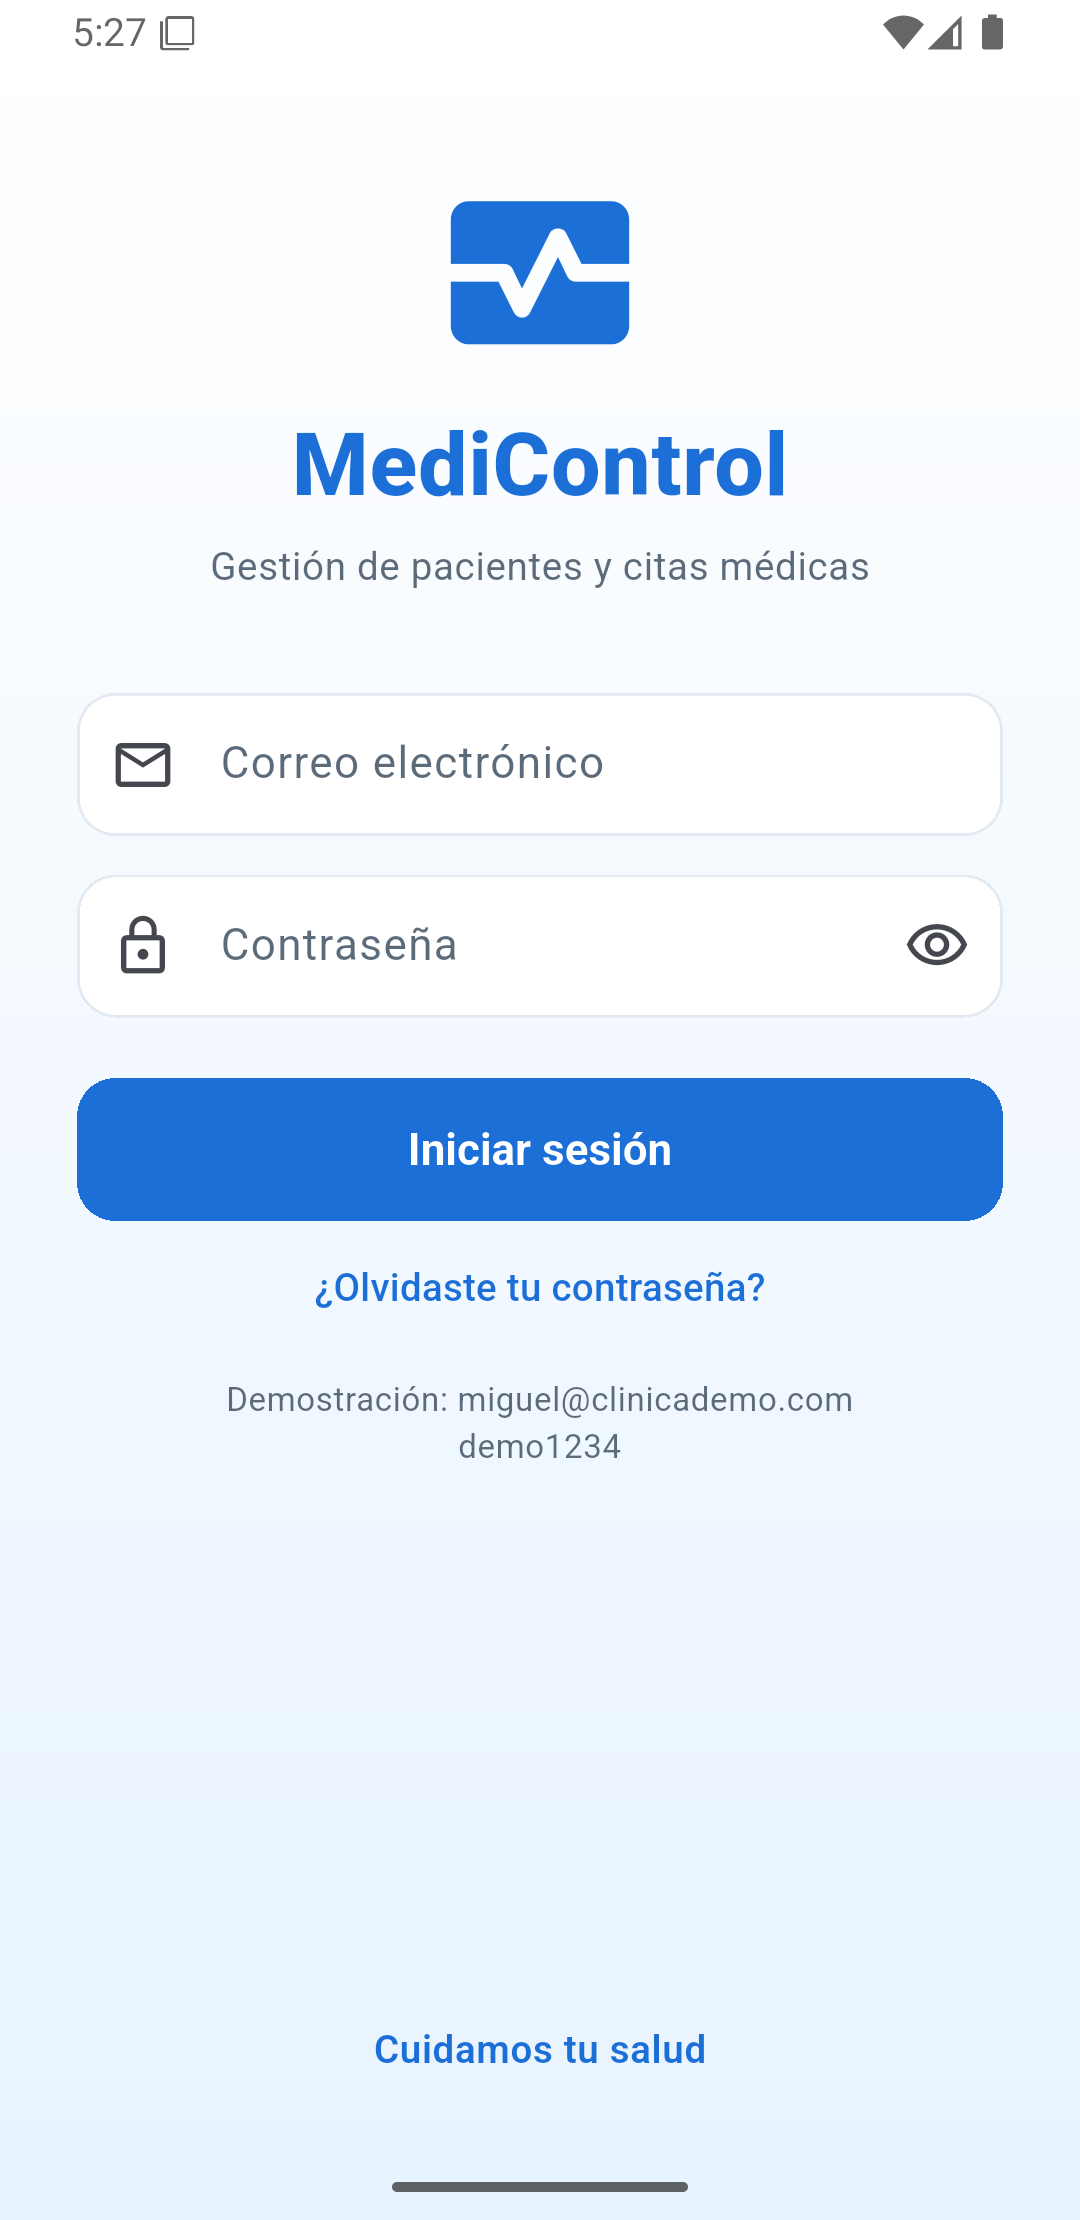
\includegraphics[width=0.15\textwidth]{medicontrol/capturas/01-login.png}\hfill
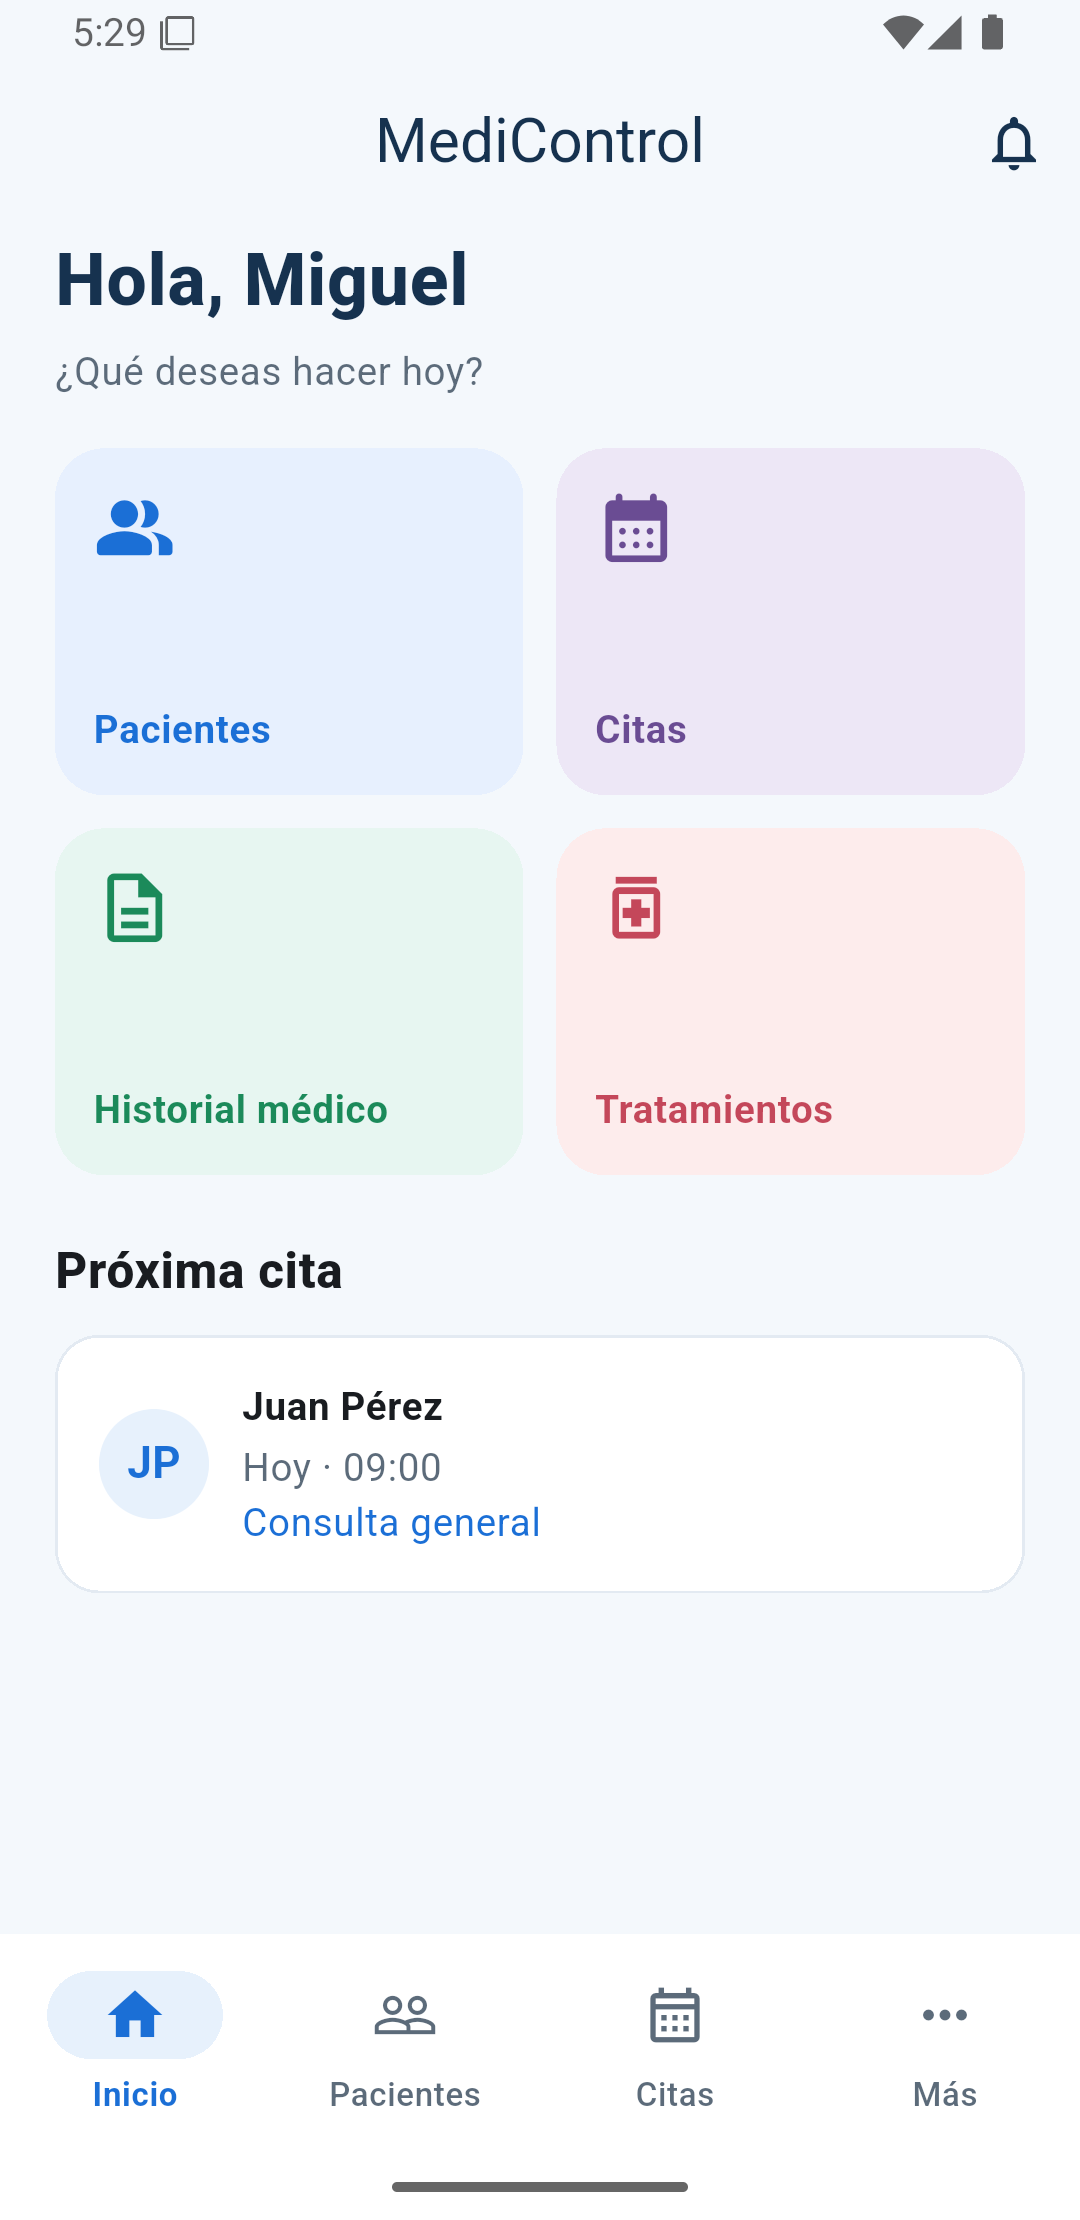
\includegraphics[width=0.15\textwidth]{medicontrol/capturas/02-inicio.png}\hfill
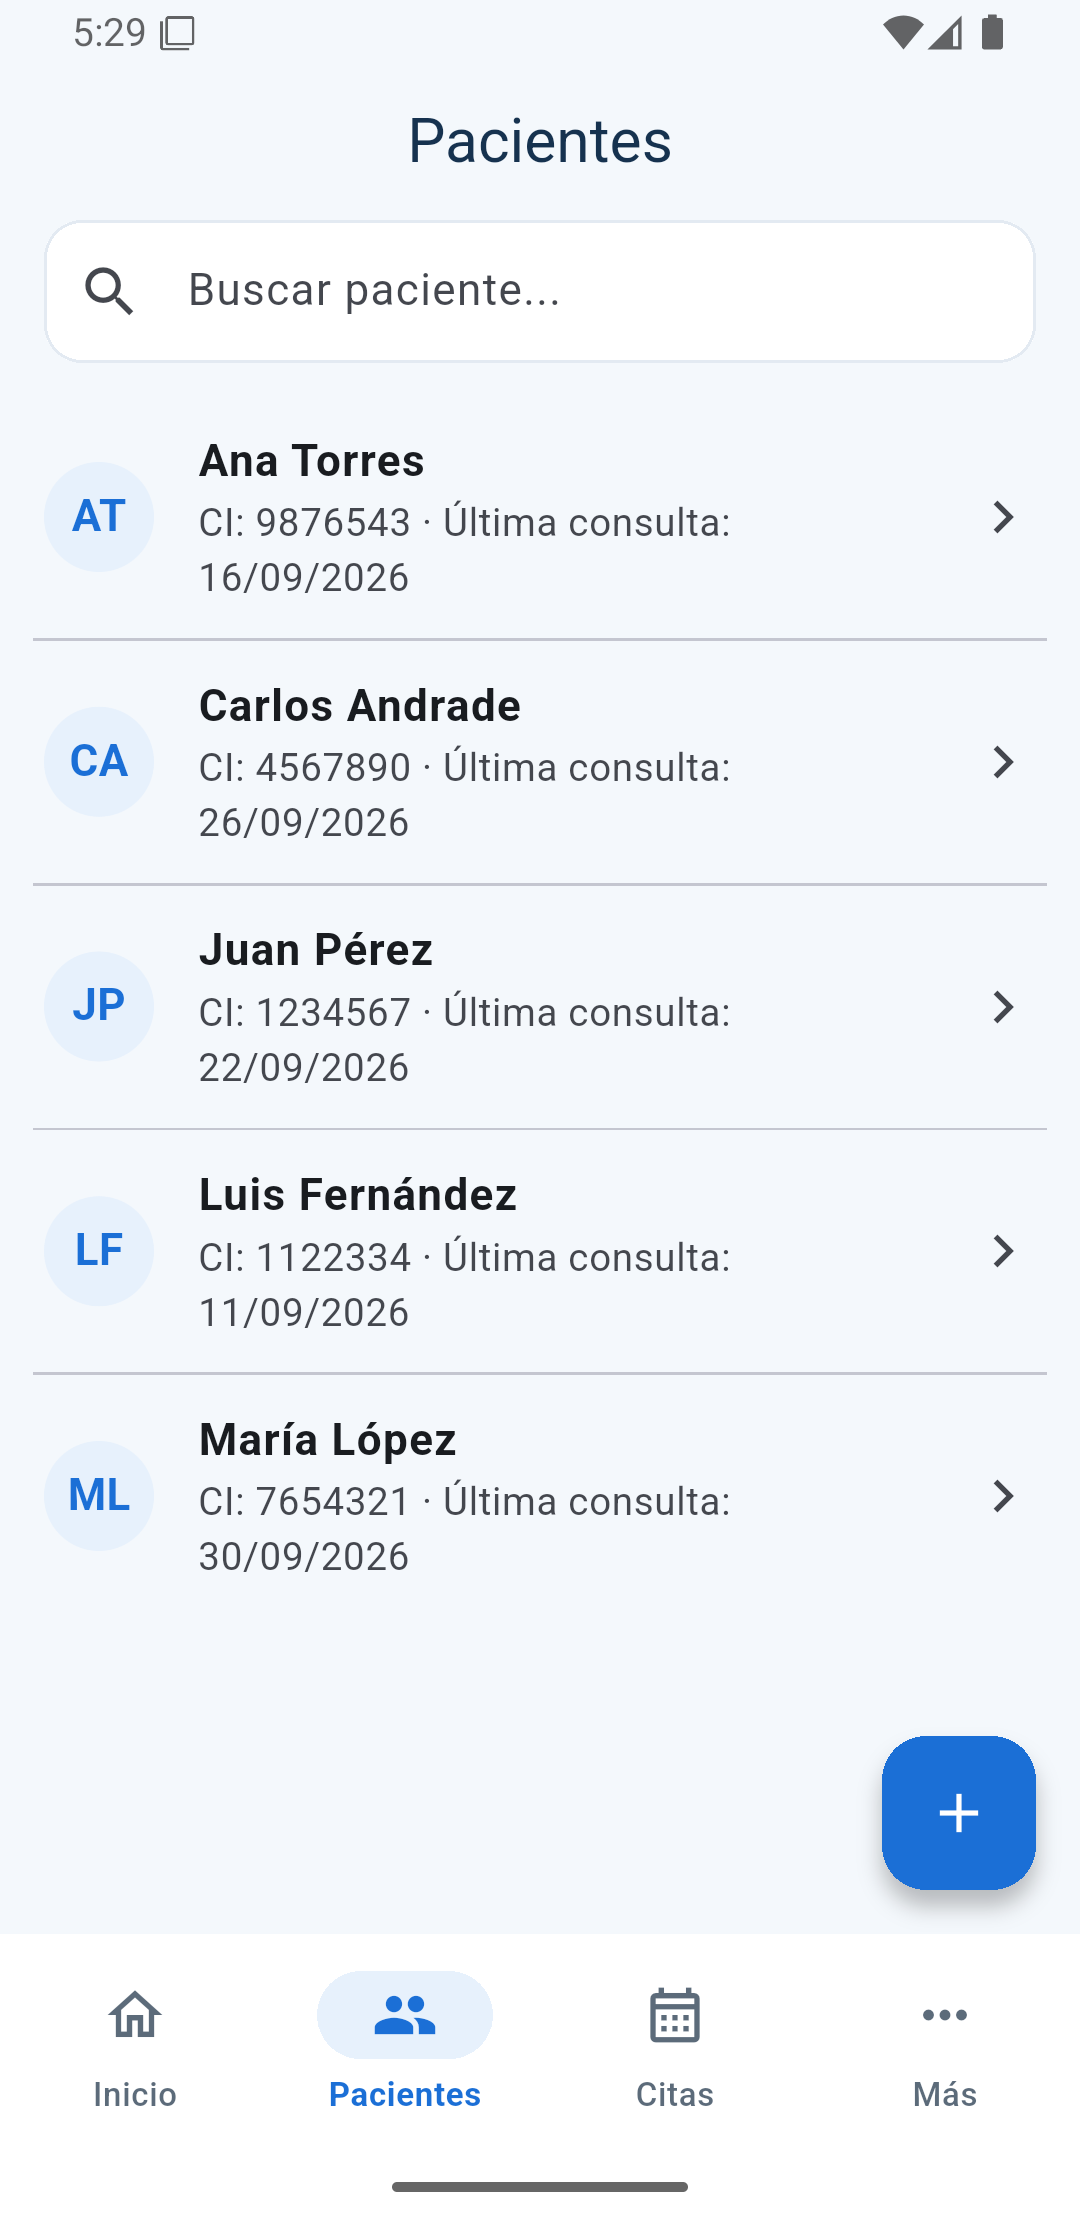
\includegraphics[width=0.15\textwidth]{medicontrol/capturas/03-pacientes.png}\hfill
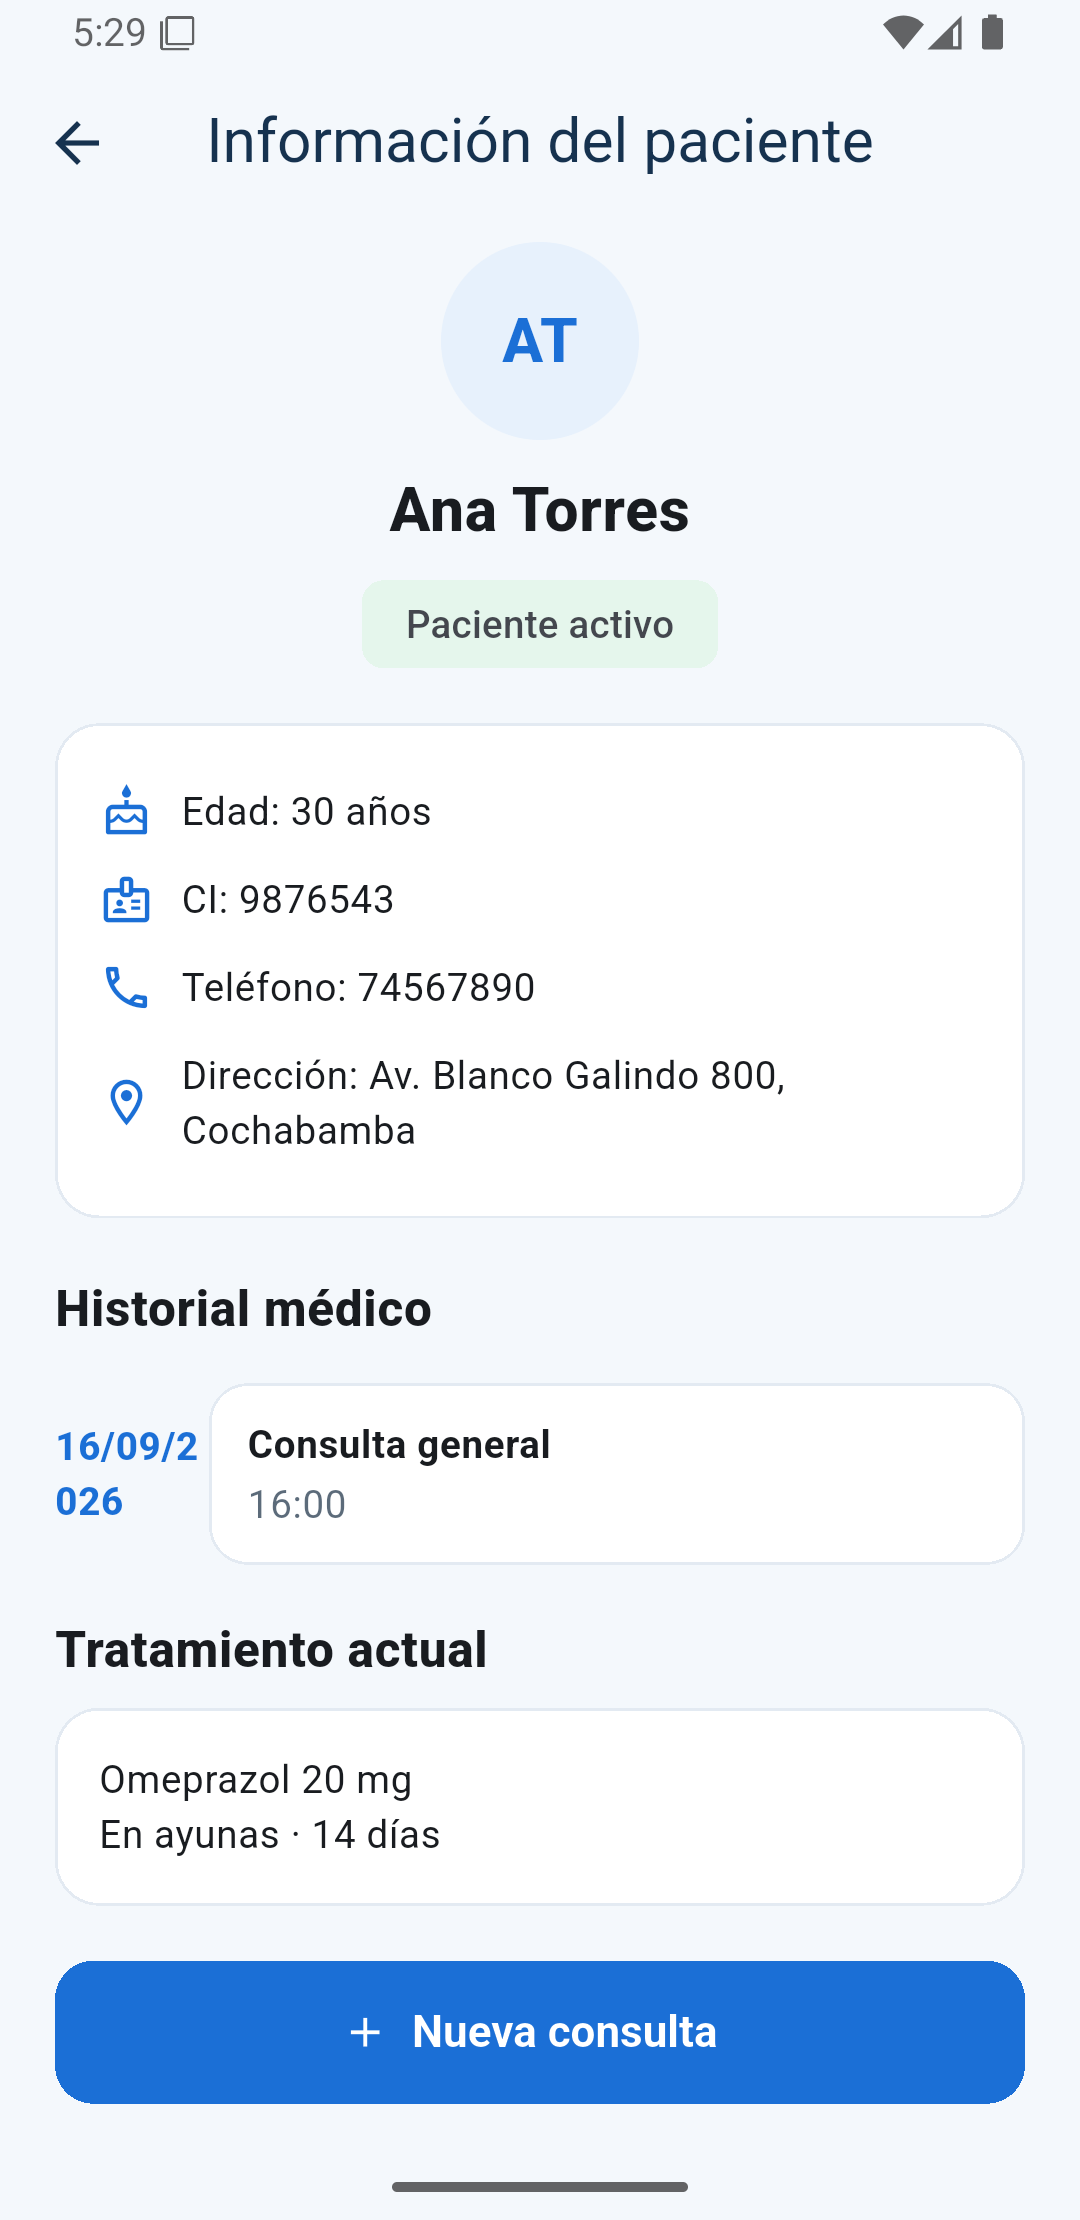
\includegraphics[width=0.15\textwidth]{medicontrol/capturas/04-ficha-ana-torres.png}\hfill
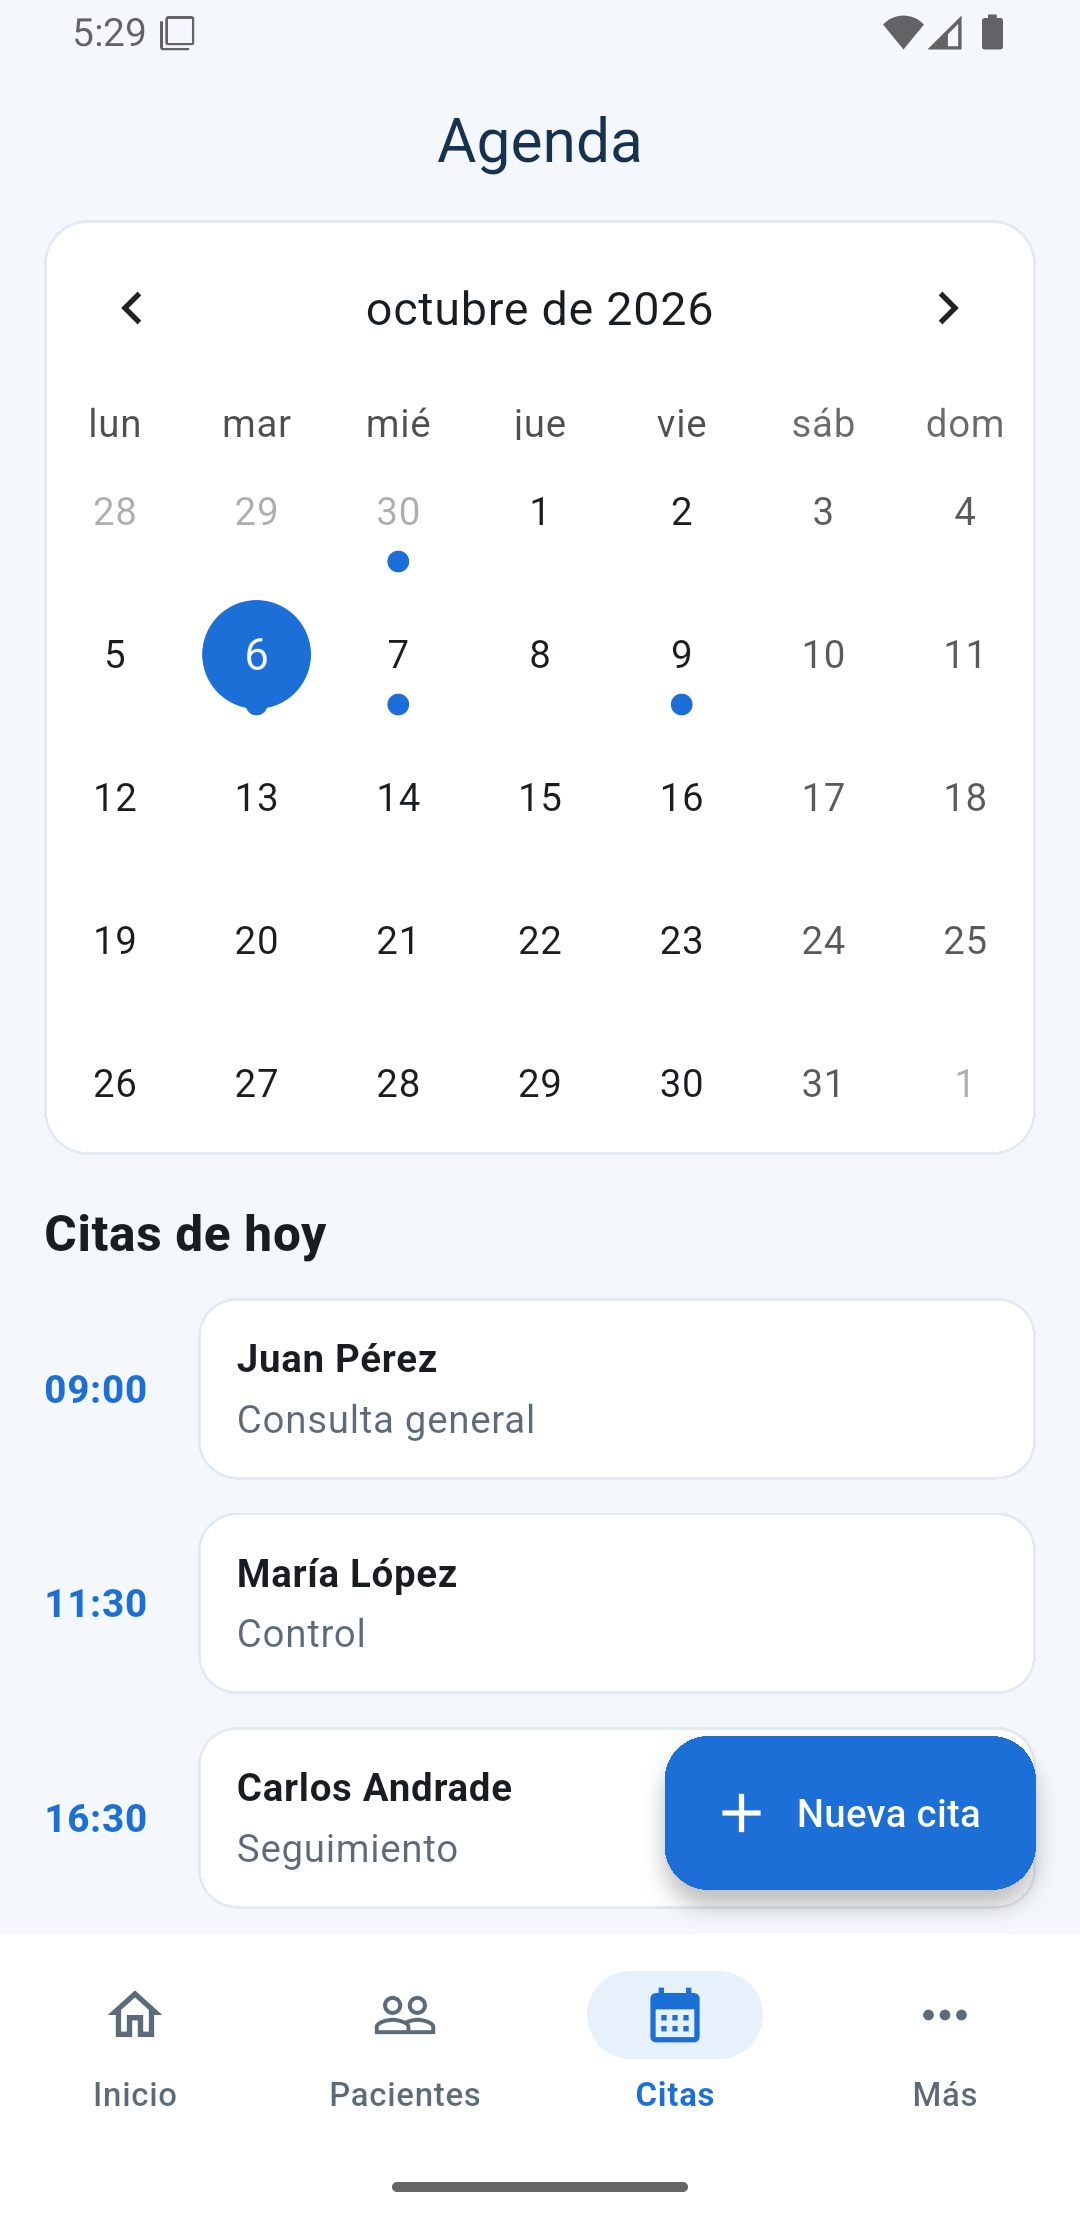
\includegraphics[width=0.15\textwidth]{medicontrol/capturas/05-agenda.png}}
\end{figure}

\section{Problemas, Trabajo Futuro y Conclusiones}

El AVD Pixel 6 se congelaba: esta entrega usa el Pixel 3a de 2 GB y el disco de datos quedó en 6 GB, no en 10.
El \path{intl} fijo, el fallo \emph{different roots} y el tope de memoria de Gradle ya quedaron en la configuración.

Queda como trabajo futuro el historial clínico editable, el CRUD de tratamientos, los recordatorios, recuperar la contraseña y la nube.
MediControl ya guarda pacientes y citas en el dispositivo, conserva la sesión y actualiza la agenda al registrar una cita.
Separar pantallas, controladores y repositorios deja listo el lugar del almacenamiento remoto.

\printbibliography

\end{document}
